\section{Comparison of results for the camera}

\subsection{Background estimation}

We will test here to what extent the estimated background is valid. For this, several series of images (taken with a video camera fixed on a support) will be used as examples.

The two steps of estimates will be analyzed: the step preceding the deblurring of determining the background from a series of images and the step that takes place each time a new image is deblurred and adapts the background dynamically.

It should also be noted that the computation time of the first step is quite high. This is due to the fact that the processing of the input (serie of images) requires the calculation of quartiles (with matlab  function quantile.m) to each element of the image matrix, which takes lots of time(sorting elements of a statistical series). It's possible, however, in the case of RGB image to significantly reduce this time by converting the images from the series in gray-scaled pictures (possible via the Graphical Users Interface).
However, we believe that this don't comprommet our bonus item. Indeed, this estimate of the background can be achieved before deblurring and is not to be recognized in the computation time(unlike the second step that updates the background during the deblurring).

\subsubsection{Before deblurring}

For each series of images, the background is estimated by applying the method of section~\ref{sec:Bg}. The goal here is to see the influence of the images provided on the final result.

The images of the first series figure~\ref{fig:AllBib} being tested were taken from a fixed support. The result is quite successful, indeed, the estimated background well matches the observed background.

\begin{figure}[h]
\centering
\begin{subfigure}{0.20\textwidth}
\includegraphics[width= \textwidth]{../Images/Camera/Human_walking/fg/IMG_3988.jpg}
\caption{}
\label{fig:Bib1}
\end{subfigure}
~
\begin{subfigure}{0.20\textwidth}
\includegraphics[{width= \textwidth}]{../Images/Camera/Human_walking/fg/IMG_3989.jpg}
\caption{}
\label{fig:Bib2}
\end{subfigure}
~
\begin{subfigure}{0.20\textwidth}
\includegraphics[{width= \textwidth}]{../Images/Camera/Human_walking/fg/IMG_3990.jpg}
\caption{}
\label{fig:Bib3}
\end{subfigure}
~
\begin{subfigure}{0.20\textwidth}
\includegraphics[{width= \textwidth}]{../Images/Camera/Human_walking/fg/IMG_3991.jpg}
\caption{}
\label{fig:Bib4}
\end{subfigure}
~
\begin{subfigure}{0.20\textwidth}
\includegraphics[{width= \textwidth}]{../Images/Camera/Human_walking/fg/IMG_3992.jpg}
\caption{}
\label{fig:Bib5}
\end{subfigure}
~
\begin{subfigure}{0.20\textwidth}
\includegraphics[{width= \textwidth}]{../Images/Camera/Human_walking/fg/IMG_3993.jpg}
\caption{}
\label{fig:Bib6}
\end{subfigure}
~
\begin{subfigure}{0.20\textwidth}
\includegraphics[{width= \textwidth}]{../Images/Camera/Human_walking/fg/IMG_3994.jpg}
\caption{}
\label{fig:Bib7}
\end{subfigure}
~
\begin{subfigure}{0.20\textwidth}
\includegraphics[{width= \textwidth}]{../Images/Camera/Human_walking/fg/IMG_3995.jpg}
\caption{}
\label{fig:Bib8}
\end{subfigure}
\caption{Images taken by camera video}
\label{fig:AllBib}
\end{figure}

\begin{figure}[h]
\centering
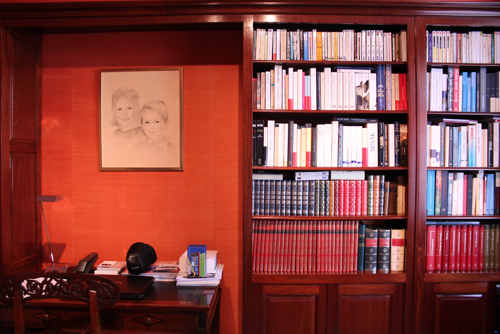
\includegraphics[{width=0.4 \textwidth}]{../Images/Camera/Human_walking/BGDetect/BGFinal.png}
\caption{Background estimation}
\label{fig:BibBG}
\end{figure} 

The second series consists of images taken by a fixed camera with a terrace figure~\ref{fig:AllTer}. The calculated background is shown on figure~\ref{fig:TerBG}. The background here is badly estimated, the center of the image is indeed altered. This result is explained by the fact that in 13 images in the series (which includes 16 photos), the foreground (the child) remains at the center of the image. So, it was integrated into the background in the calculated mean.


\begin{figure}[h]
\centering
\begin{subfigure}{0.20\textwidth}
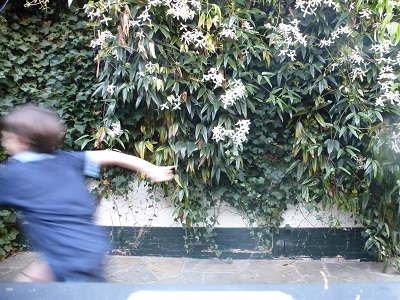
\includegraphics[width= \textwidth]{../Images/Camera/Terasse/fg/P1030014.jpg}
\caption{}
\label{fig:Ter1}
\end{subfigure}
~
\begin{subfigure}{0.20\textwidth}
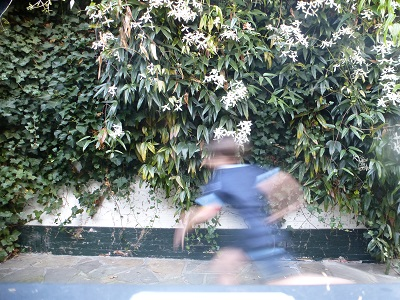
\includegraphics[{width= \textwidth}]{../Images/Camera/Terasse/fg/P1030015.jpg}
\caption{}
\label{fig:Ter2}
\end{subfigure}
~
\begin{subfigure}{0.20\textwidth}
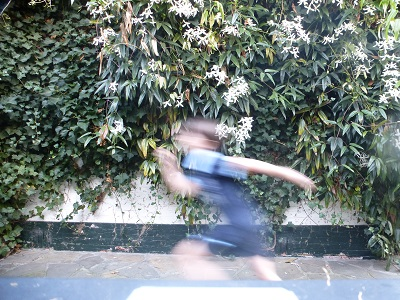
\includegraphics[{width= \textwidth}]{../Images/Camera/Terasse/fg/P1030016.jpg}
\caption{}
\label{fig:Ter3}
\end{subfigure}
~
\begin{subfigure}{0.20\textwidth}
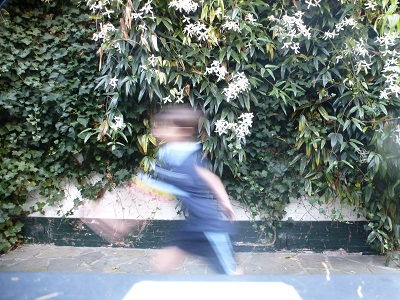
\includegraphics[{width= \textwidth}]{../Images/Camera/Terasse/fg/P1030017.jpg}
\caption{}
\label{fig:Ter4}
\end{subfigure}
~
\begin{subfigure}{0.20\textwidth}
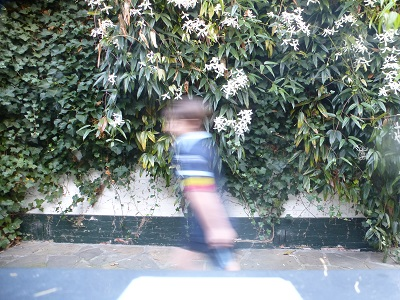
\includegraphics[{width= \textwidth}]{../Images/Camera/Terasse/fg/P1030018.jpg}
\caption{}
\label{fig:Ter5}
\end{subfigure}
~
\begin{subfigure}{0.20\textwidth}
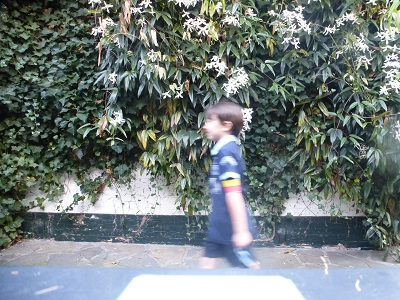
\includegraphics[{width= \textwidth}]{../Images/Camera/Terasse/fg/P1030019.jpg}
\caption{}
\label{fig:Ter6}
\end{subfigure}
~
\begin{subfigure}{0.20\textwidth}
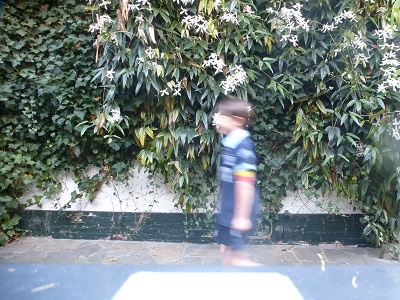
\includegraphics[{width= \textwidth}]{../Images/Camera/Terasse/fg/P1030020.jpg}
\caption{}
\label{fig:Ter7}
\end{subfigure}
~
\begin{subfigure}{0.20\textwidth}
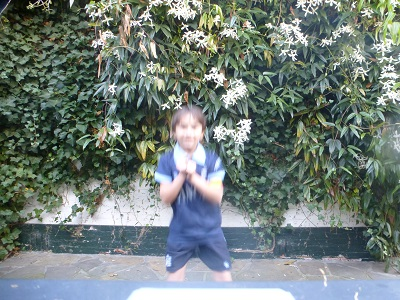
\includegraphics[{width= \textwidth}]{../Images/Camera/Terasse/fg/P1030021.jpg}
\caption{}
\label{fig:Ter8}
\end{subfigure}
~
\begin{subfigure}{0.20\textwidth}
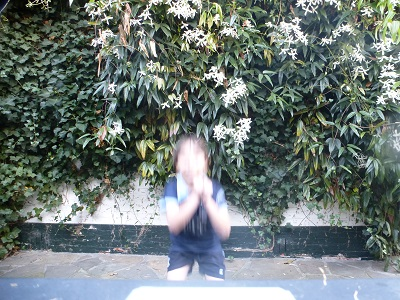
\includegraphics[{width= \textwidth}]{../Images/Camera/Terasse/fg/P1030022.jpg}
\caption{}
\label{fig:Ter9}
\end{subfigure}
~
\begin{subfigure}{0.20\textwidth}
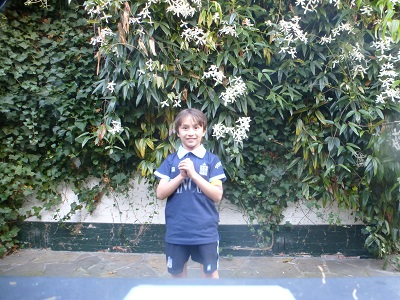
\includegraphics[{width= \textwidth}]{../Images/Camera/Terasse/fg/P1030023.jpg}
\caption{}
\label{Ter10}
\end{subfigure}
~
\begin{subfigure}{0.20\textwidth}
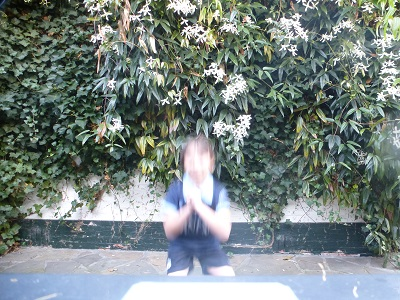
\includegraphics[{width= \textwidth}]{../Images/Camera/Terasse/fg/P1030024.jpg}
\caption{}
\label{fig:Ter11}
\end{subfigure}
~
\begin{subfigure}{0.20\textwidth}
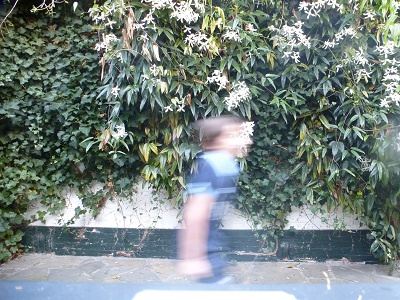
\includegraphics[{width= \textwidth}]{../Images/Camera/Terasse/fg/P1030025.jpg}
\caption{}
\label{fig:Ter12}
\end{subfigure}
~
\begin{subfigure}{0.20\textwidth}
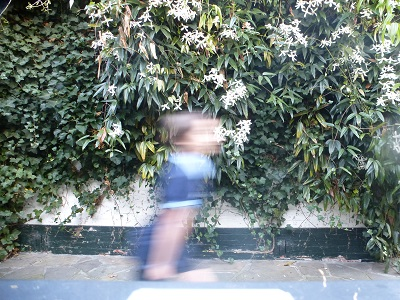
\includegraphics[{width= \textwidth}]{../Images/Camera/Terasse/fg/P1030026.jpg}
\caption{}
\label{fig:Ter13}
\end{subfigure}
~
\begin{subfigure}{0.20\textwidth}
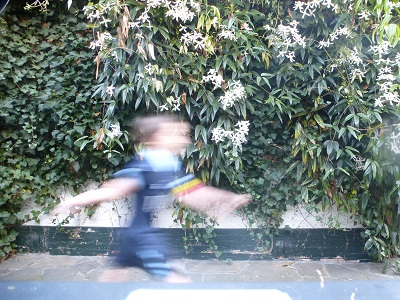
\includegraphics[{width= \textwidth}]{../Images/Camera/Terasse/fg/P1030027.jpg}
\caption{}
\label{fig:Ter14}
\end{subfigure}
~
\begin{subfigure}{0.20\textwidth}
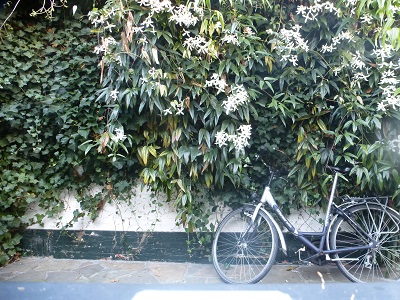
\includegraphics[{width= \textwidth}]{../Images/Camera/Terasse/fg/P1030028.jpg}
\caption{}
\label{fig:Ter15}
\end{subfigure}
~
\begin{subfigure}{0.20\textwidth}
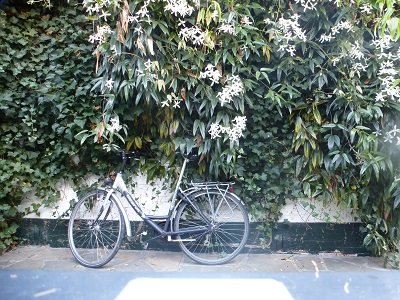
\includegraphics[{width= \textwidth}]{../Images/Camera/Terasse/fg/P1030029.jpg}
\caption{}
\label{fig:Ter16}
\end{subfigure}
\caption{Images taken by camera video}
\label{fig:AllTer}
\end{figure}

\begin{figure}[h]
\centering
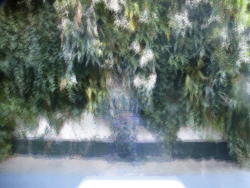
\includegraphics[{width=0.4 \textwidth}]{../Images/Camera/Terasse/BGDetect/BG.png}
\label{fig:TerBG}
\caption{Background estimation}
\end{figure} 

\subsubsection{Udpade Background}
\label{subsec:UdpadeBg}

For each new image, the foreground will be deblurred thanks to the background. It is therefore essential that it be changed dynamically when pictures are received (we assume that the pictures follow in chronological order). This requires giving some weight to the new image in the calculation of the new background. Indeed, the background should not be updated in the same way if two pictures follow of $1$ [s] or of $10$ [min], it will assign a larger weight to the new image in the second case. This weight depends on the parameter $a$ explained above (see ~\ref{sec:Bg}). Figures \ref{fig:AllAut}, \ref{fig:AutBG} and \ref{} clearly show the influence of this parameter on the different Background. A Serie of images of a motorway is used to estimate the background (figure~\ref{fig:AllAut}) and the result is shown in figure~\ref{fig:AutBG}. After, the initial serie is used to udpade the background estimation. We do it with $a=0.5$ as shown in \ref{fig:Udpade}.

\begin{figure}[h]
\centering
\begin{subfigure}{0.20\textwidth}
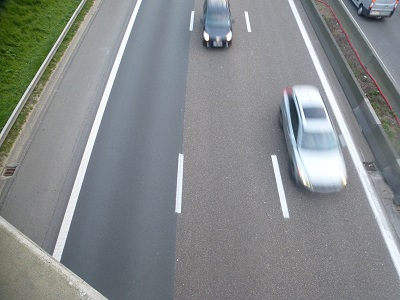
\includegraphics[width= \textwidth]{../Images/Camera/Autoroute/fg/06.jpg}
\caption{}
\label{fig:Aut1}
\end{subfigure}
~
\begin{subfigure}{0.20\textwidth}
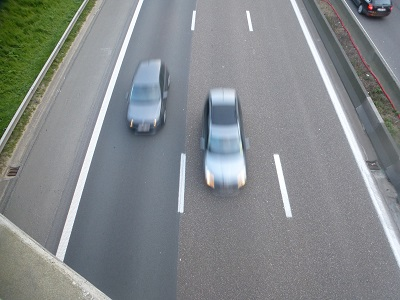
\includegraphics[{width= \textwidth}]{../Images/Camera/Autoroute/fg/07.jpg}
\caption{}
\label{fig:Aut2}
\end{subfigure}
~
\begin{subfigure}{0.20\textwidth}
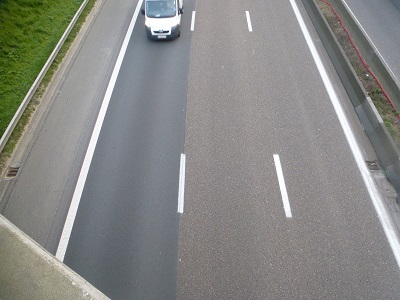
\includegraphics[{width= \textwidth}]{../Images/Camera/Autoroute/fg/08.jpg}
\caption{}
\label{fig:Aut3}
\end{subfigure}
~
\begin{subfigure}{0.20\textwidth}
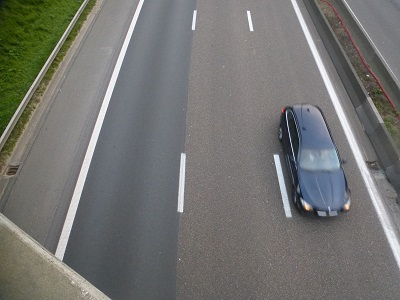
\includegraphics[{width= \textwidth}]{../Images/Camera/Autoroute/fg/09.jpg}
\caption{}
\label{fig:Aut4}
\end{subfigure}
~
\begin{subfigure}{0.20\textwidth}
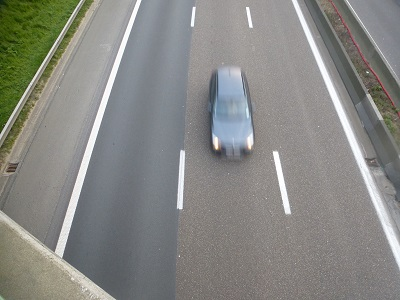
\includegraphics[{width= \textwidth}]{../Images/Camera/Autoroute/fg/10.jpg}
\caption{}
\label{fig:Aut5}
\end{subfigure}
~
\begin{subfigure}{0.20\textwidth}
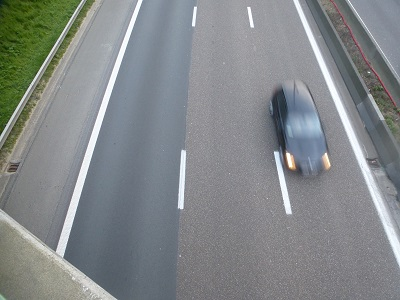
\includegraphics[{width= \textwidth}]{../Images/Camera/Autoroute/fg/11.jpg}
\caption{}
\label{fig:Aut6}
\end{subfigure}
~
\begin{subfigure}{0.20\textwidth}
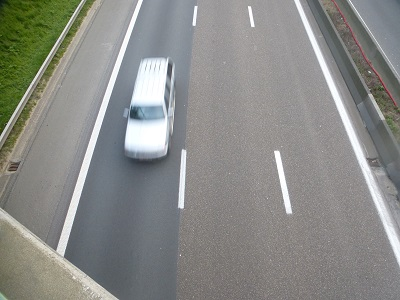
\includegraphics[{width= \textwidth}]{../Images/Camera/Autoroute/fg/12.jpg}
\caption{}
\label{fig:Aut7}
\end{subfigure}
~
\begin{subfigure}{0.20\textwidth}
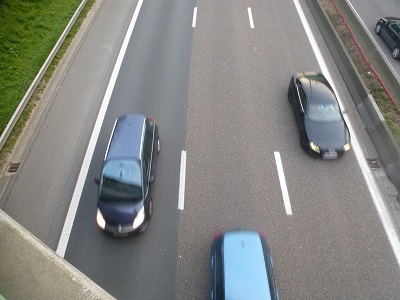
\includegraphics[{width= \textwidth}]{../Images/Camera/Autoroute/fg/13.jpg}
\caption{}
\label{fig:Aut8}
\end{subfigure}
~
\begin{subfigure}{0.20\textwidth}
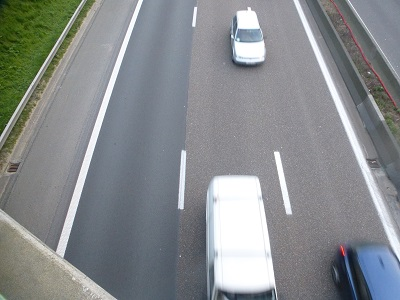
\includegraphics[{width= \textwidth}]{../Images/Camera/Autoroute/fg/14.jpg}
\caption{}
\label{fig:Aut9}
\end{subfigure}
~
\begin{subfigure}{0.20\textwidth}
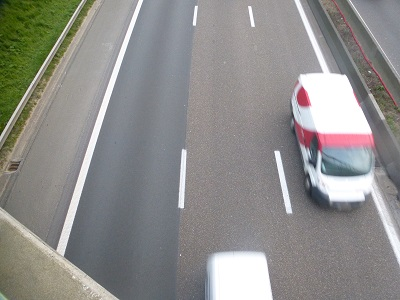
\includegraphics[{width= \textwidth}]{../Images/Camera/Autoroute/fg/15.jpg}
\caption{}
\label{Aut10}
\end{subfigure}
~
\begin{subfigure}{0.20\textwidth}
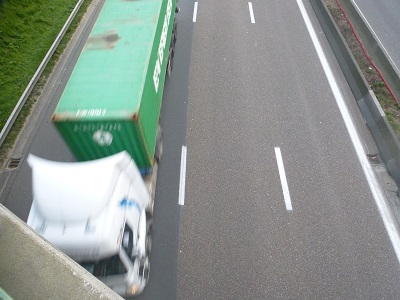
\includegraphics[{width= \textwidth}]{../Images/Camera/Autoroute/fg/16.jpg}
\caption{}
\label{fig:Aut11}
\end{subfigure}
\caption{Images taken by camera video}
\label{fig:AllAut}
\end{figure}

\begin{figure}[h]
\centering
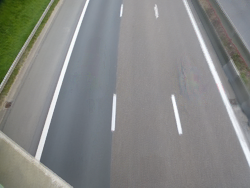
\includegraphics[{width=0.4 \textwidth}]{../Images/Camera/Autoroute/BGDetect/BGDetect.png}
\label{fig:AutBG}
\caption{Background estimation}
\end{figure} 


\begin{figure}[h]
\centering
\begin{subfigure}{0.20\textwidth}
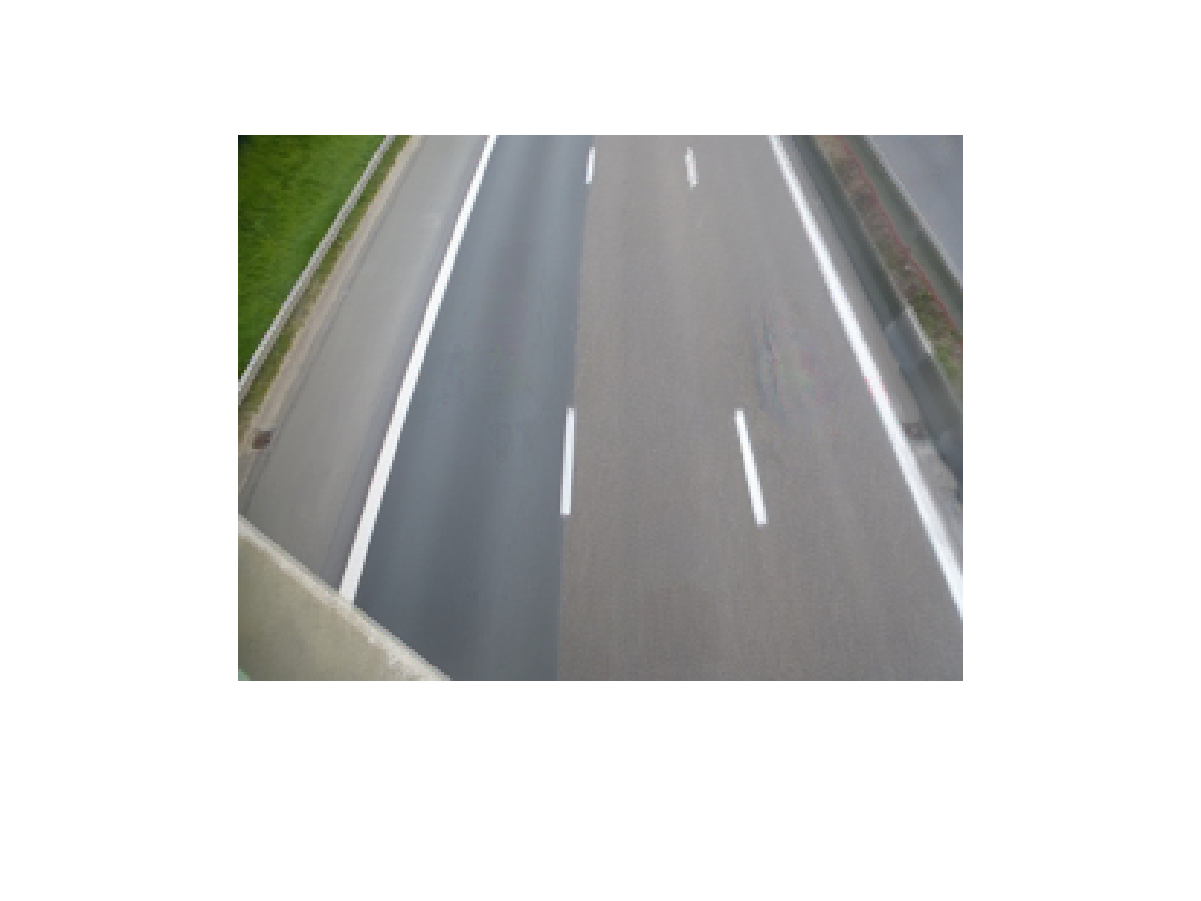
\includegraphics[width= \textwidth]{../Images/Camera/Autoroute/fg/a50/CamDeblurred-1.png}
\caption{}
\label{fig:UAut1}
\end{subfigure}
~
\begin{subfigure}{0.20\textwidth}
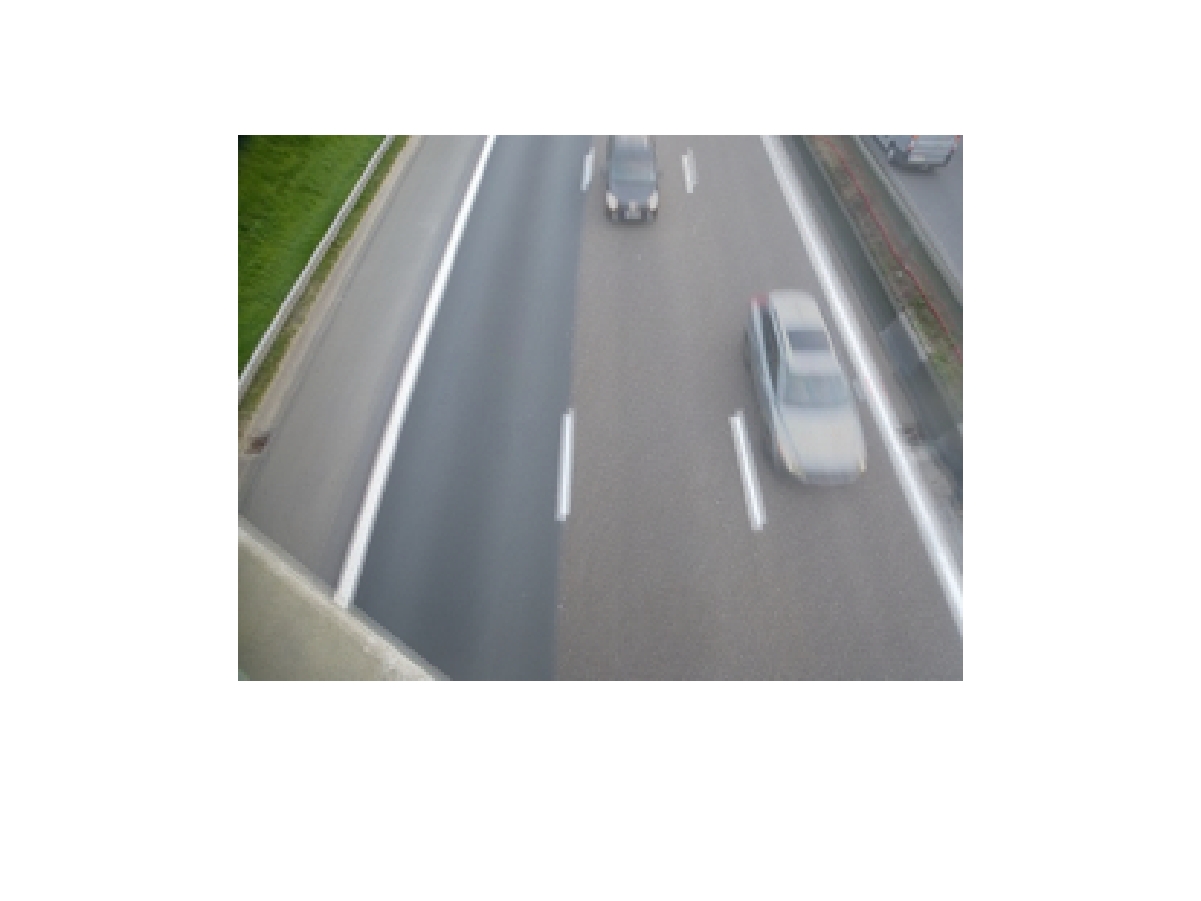
\includegraphics[{width= \textwidth}]{../Images/Camera/Autoroute/fg/a50/CamDeblurred-2.png}
\caption{}
\label{fig:UAut2}
\end{subfigure}
~
\begin{subfigure}{0.20\textwidth}
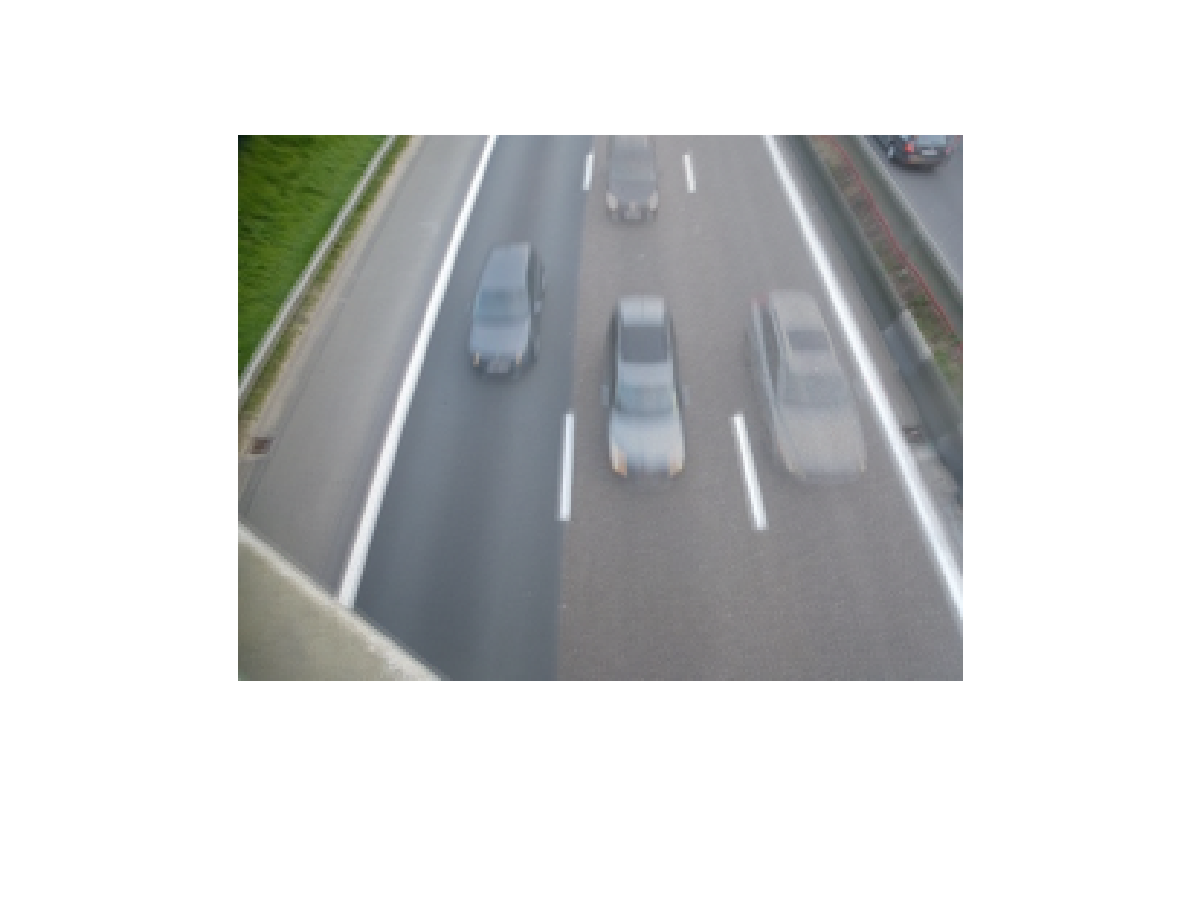
\includegraphics[{width= \textwidth}]{../Images/Camera/Autoroute/fg/a50/CamDeblurred-3.png}
\caption{}
\label{fig:UAut3}
\end{subfigure}
~
\begin{subfigure}{0.20\textwidth}
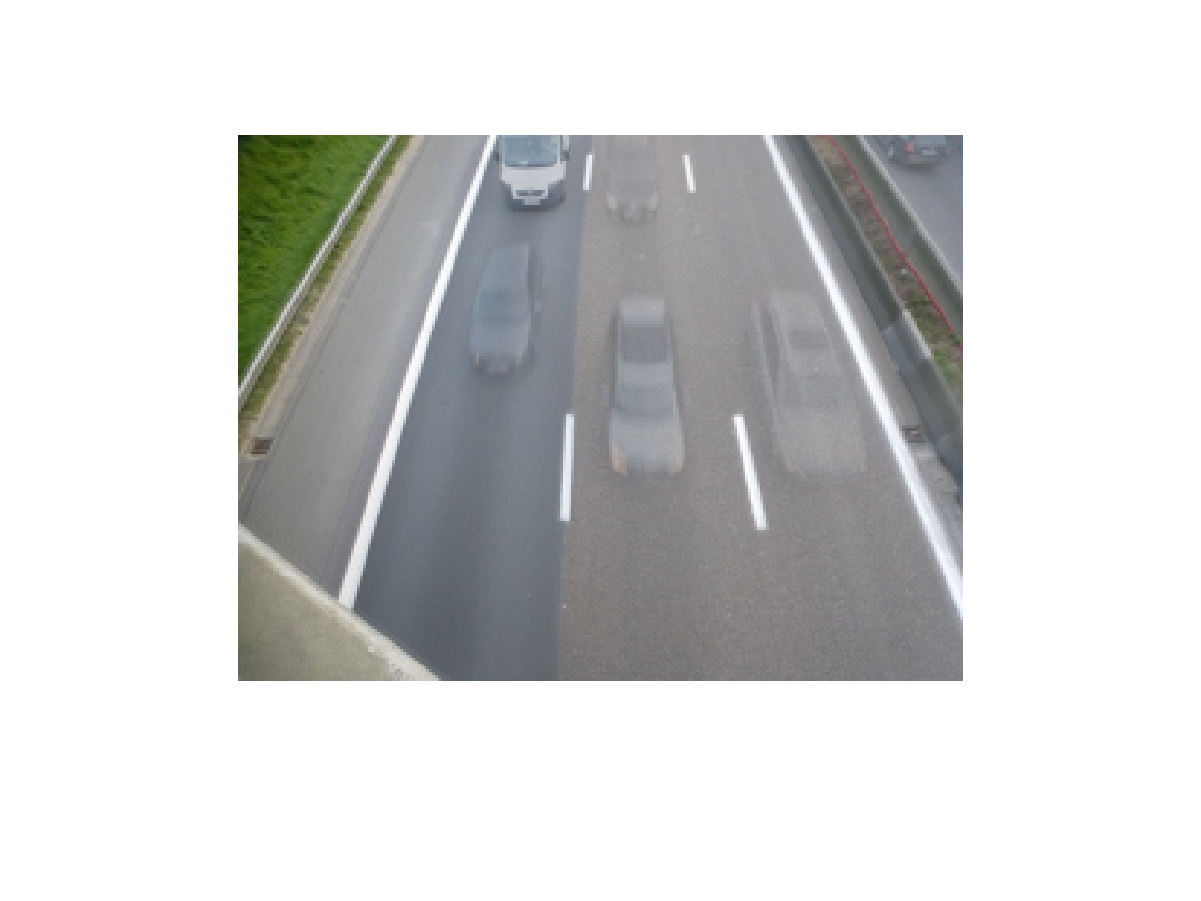
\includegraphics[{width= \textwidth}]{../Images/Camera/Autoroute/fg/a50/CamDeblurred-4.png}
\caption{}
\label{fig:UAut4}
\end{subfigure}
~
\begin{subfigure}{0.20\textwidth}
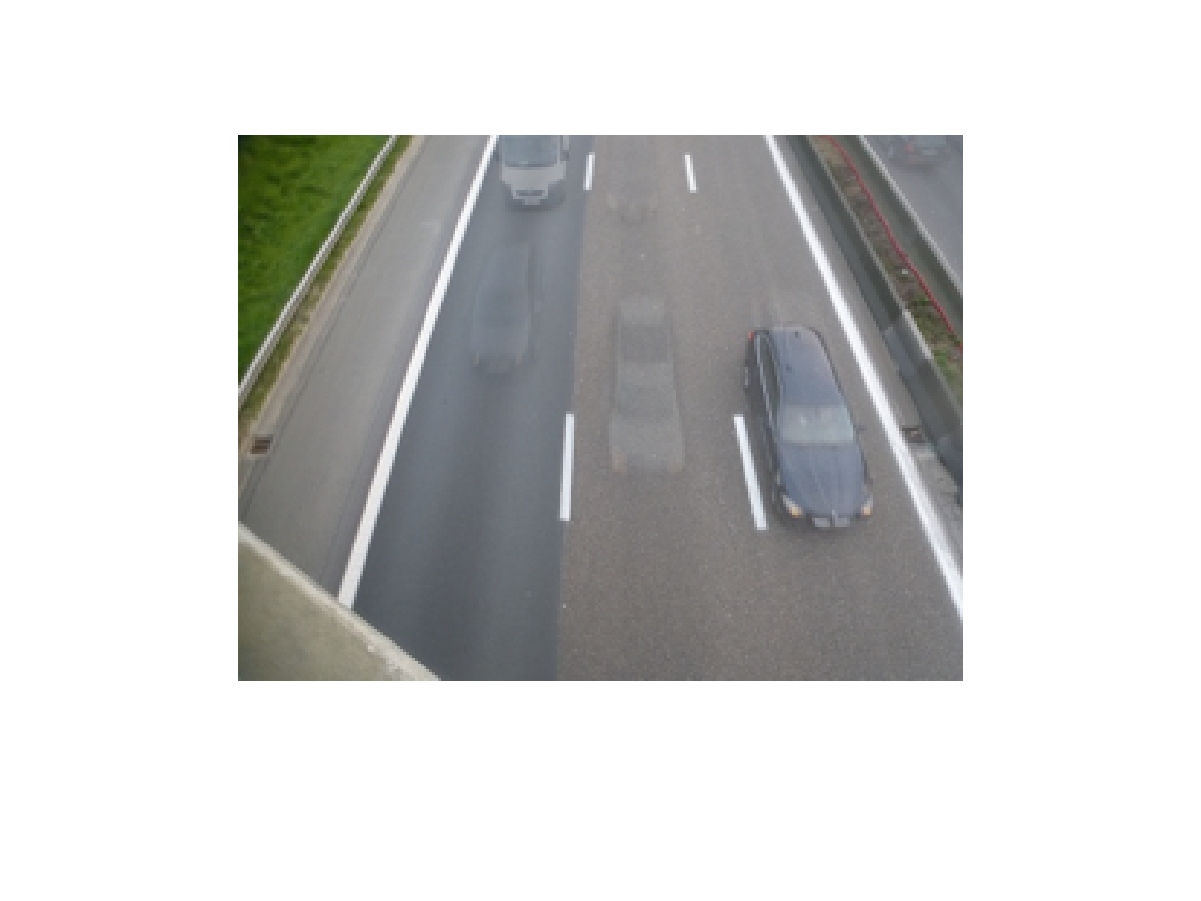
\includegraphics[{width= \textwidth}]{../Images/Camera/Autoroute/fg/a50/CamDeblurred-5.png}
\caption{}
\label{fig:UAut5}
\end{subfigure}
~
\begin{subfigure}{0.20\textwidth}
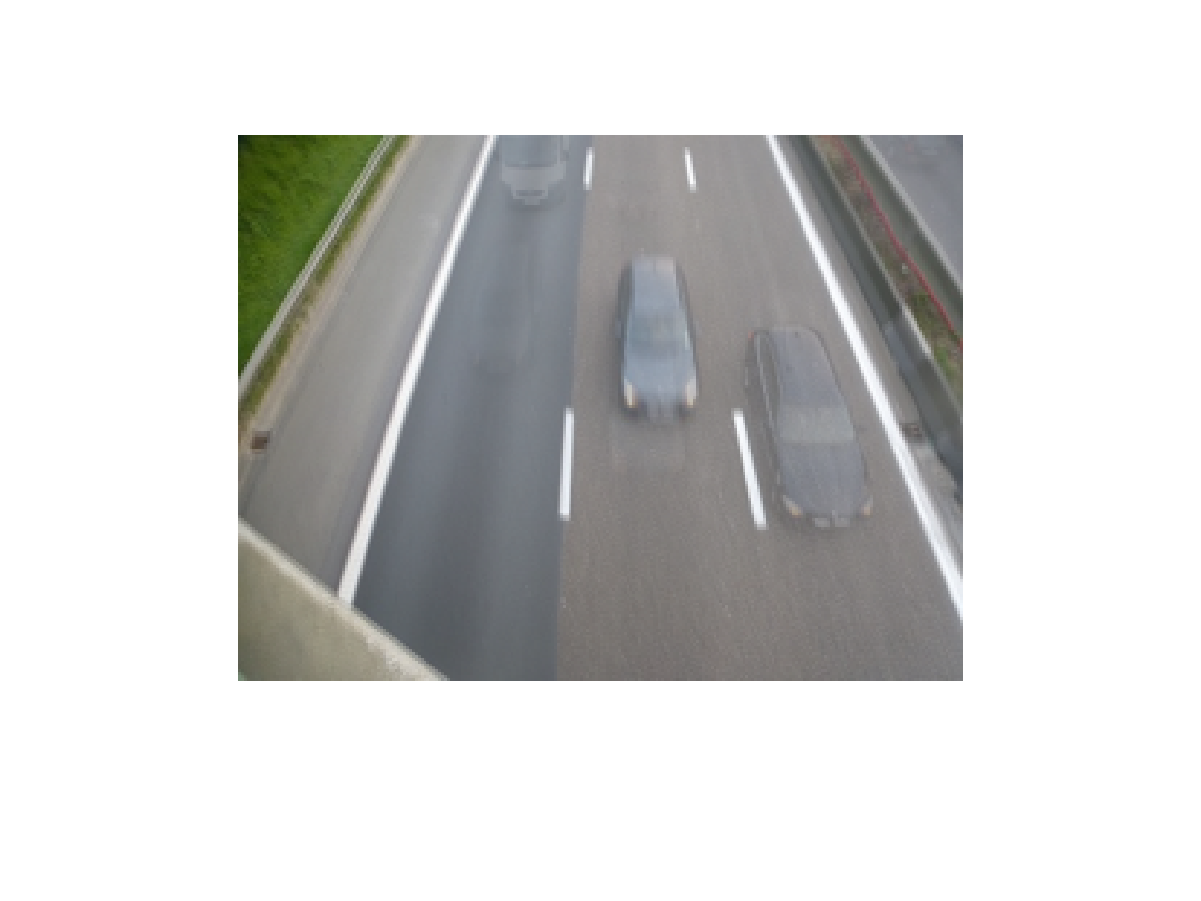
\includegraphics[{width= \textwidth}]{../Images/Camera/Autoroute/fg/a50/CamDeblurred-6.png}
\caption{}
\label{fig:UAut6}
\end{subfigure}
~
\begin{subfigure}{0.20\textwidth}
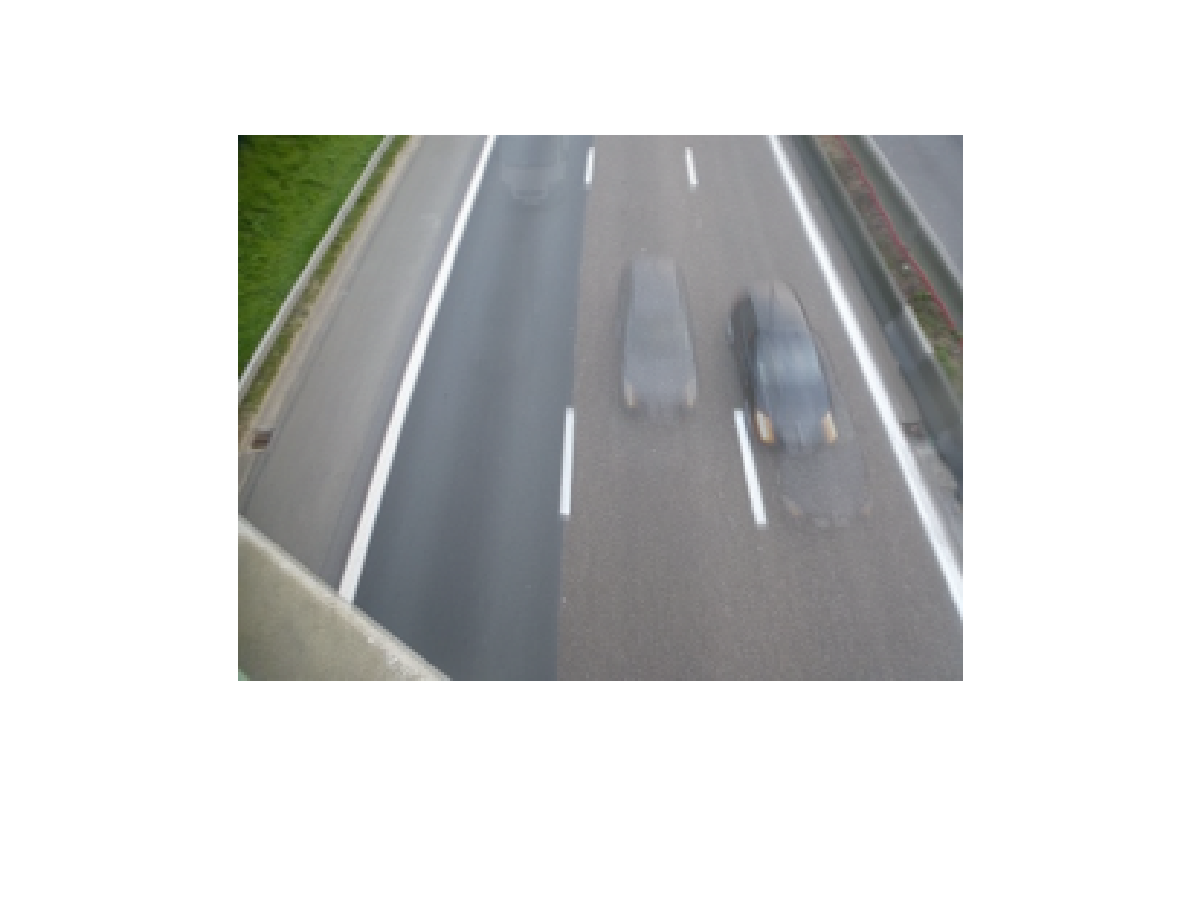
\includegraphics[{width= \textwidth}]{../Images/Camera/Autoroute/fg/a50/CamDeblurred-7.png}
\caption{}
\label{fig:UAut7}
\end{subfigure}
~
\begin{subfigure}{0.20\textwidth}
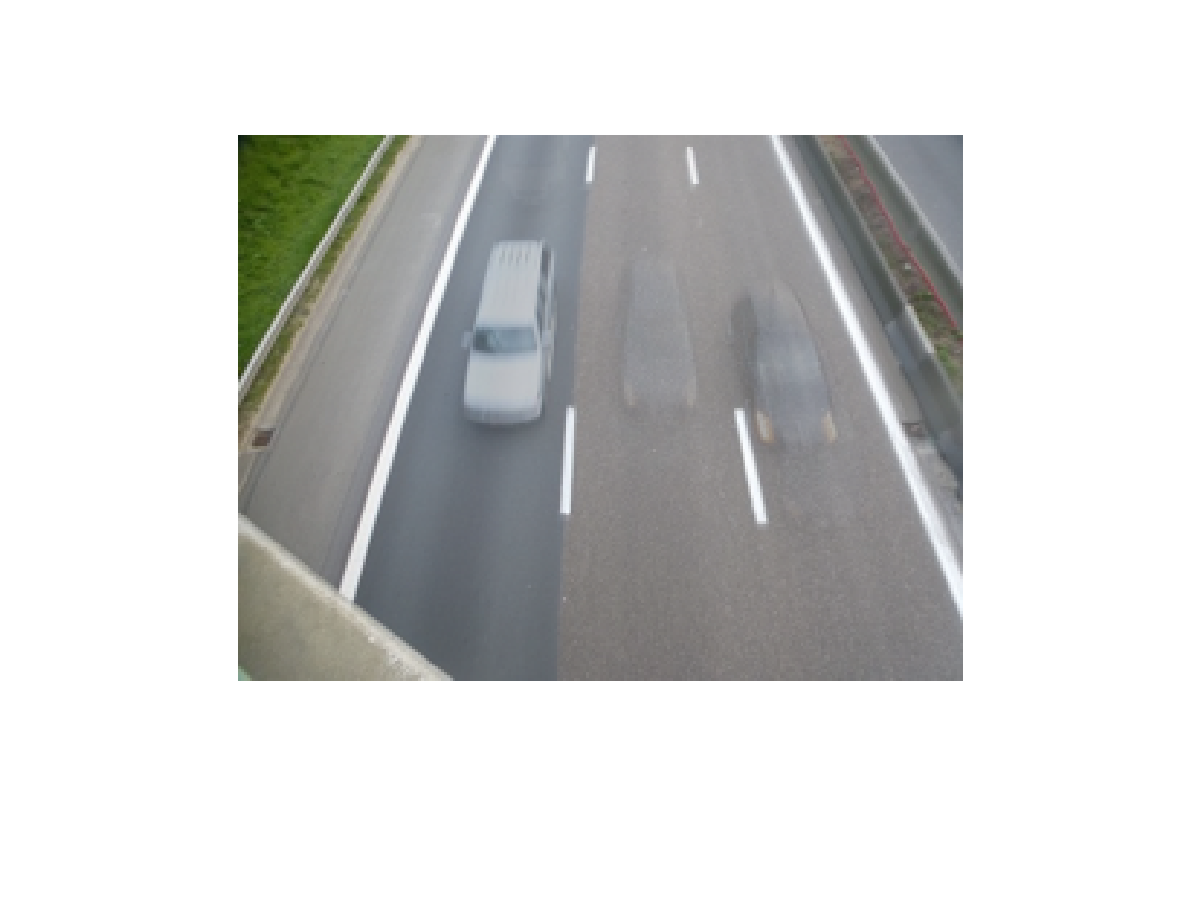
\includegraphics[{width= \textwidth}]{../Images/Camera/Autoroute/fg/a50/CamDeblurred-8.png}
\caption{}
\label{fig:UAut8}
\end{subfigure}
~
\begin{subfigure}{0.20\textwidth}
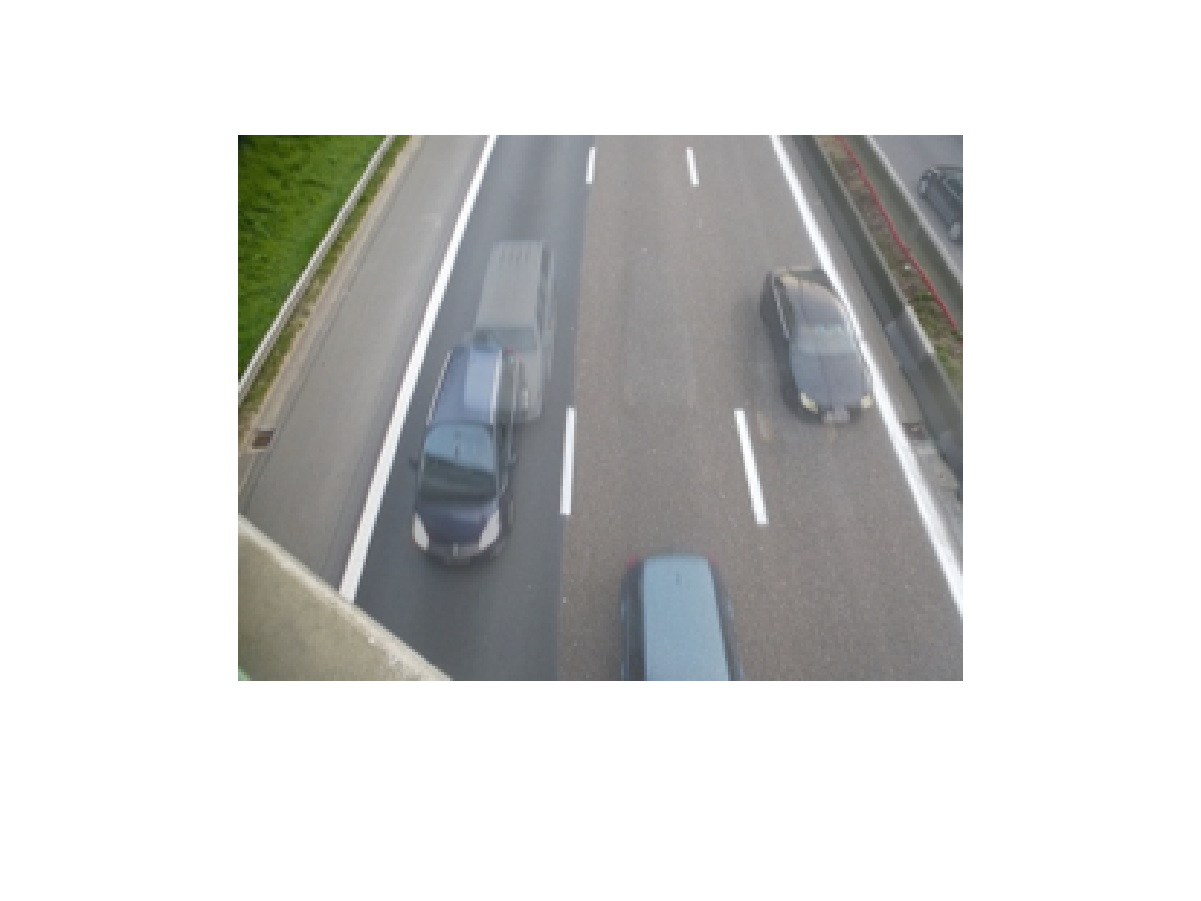
\includegraphics[{width= \textwidth}]{../Images/Camera/Autoroute/fg/a50/CamDeblurred-9.png}
\caption{}
\label{fig:UAut9}
\end{subfigure}
~
\begin{subfigure}{0.20\textwidth}
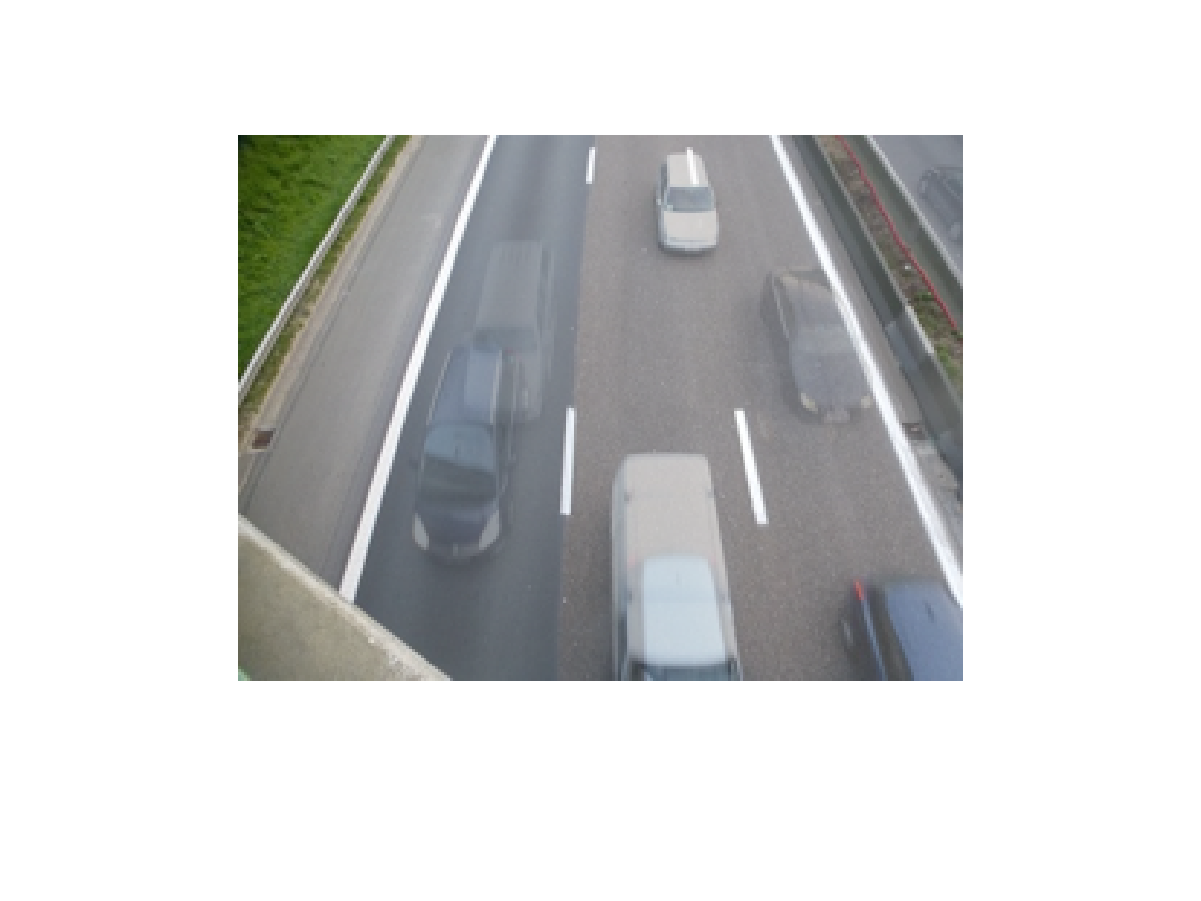
\includegraphics[{width= \textwidth}]{../Images/Camera/Autoroute/fg/a50/CamDeblurred-10.png}
\caption{}
\label{fig:UAut10}
\end{subfigure}
~
\begin{subfigure}{0.20\textwidth}
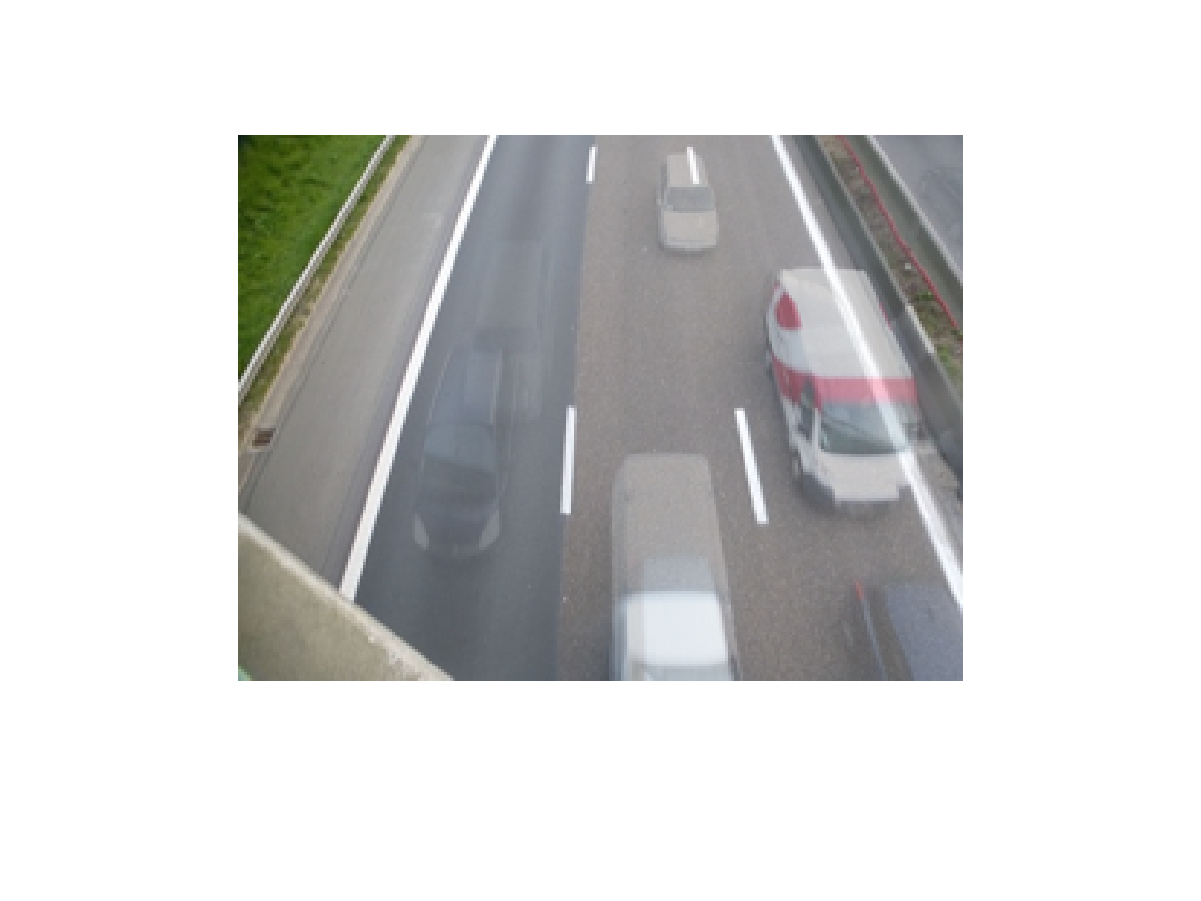
\includegraphics[{width= \textwidth}]{../Images/Camera/Autoroute/fg/a50/CamDeblurred-11.png}
\caption{}
\label{fig:UAut11}
\end{subfigure}
\caption{Udpade of the Background with $a=0.5$}
\label{fig:Udpade}
\end{figure}

It's not very realistic to update the background but the example is interesting to see the influence of the parameter. Taking $a = 0.99$ (value taken by default), changes in the background are very low and not percpectibles to the naked eye. However, for a sufficiently large sample (hundreds of pictures for a real camera surveillance), the background will change even with $a=0.99$. 

\subsection{Deblurring}
Let's start with simple rectangles with the \figref{dontpanic}.
We can see with \figref{dontpanic-40-0_2_1-20} and \figref{dontpanic-40-0_2_1-20}
that ``select-lucy'' has borders problems that get worse at
each iteration.
That shows that increasing the number of iteration
is not always a good idea since it make the errors spread.
This is the same scenerio for \figref{dontpanic_blue-40-0_2_1-20}
and \figref{dontpanic_blue-40-0_2_1-60}.
This problem was expected since the resolution at the border
is an approximation that is a bit wrong so it creates errors.

\begin{myfig}{dontpanic}{Square image on real background blurred with $(40,\ang{0})$}
  \begin{myfigsub}{dontpanic-40-0_2_1-20}
    {``select-lucy'' with 20 iterations}{0.49}
    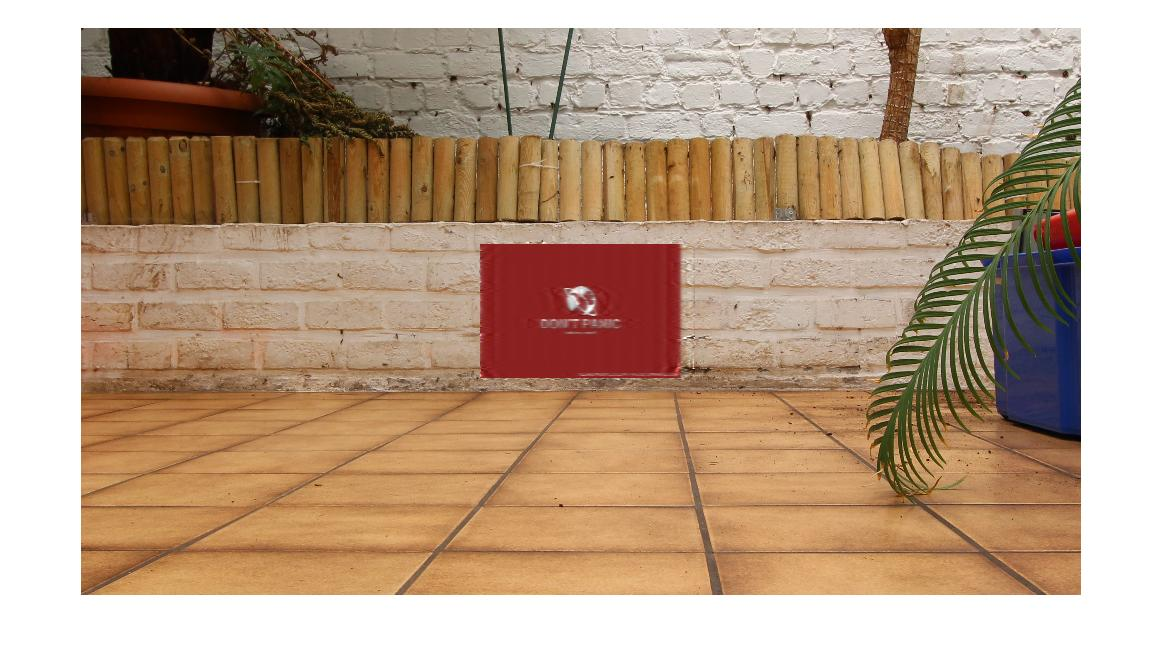
\includegraphics[trim=15cm 7cm 15cm 7cm,clip,width=\textwidth]{dontpanic-40_0-2_1-20.jpg}
  \end{myfigsub}
  \begin{myfigsub}{dontpanic-40-0_2_1-100}
    {``select-lucy'' with 100 iterations}{0.49}
    \includegraphics[trim=15cm 7cm 15cm 7cm,clip,width=\textwidth]{dontpanic-40_0-2_1-100.jpg}
  \end{myfigsub}
  \begin{myfigsub}{dontpanic-40-0_2_2-20}
    {``exact-lucy'' with 20 iterations}{0.49}
    \includegraphics[trim=15cm 7cm 15cm 7cm,clip,width=\textwidth]{dontpanic-40_0-2_2-20.jpg}
  \end{myfigsub}
  \begin{myfigsub}{dontpanic-40-0_2_2-100}
    {``exact-lucy'' with 100 iterations}{0.49}
    \includegraphics[trim=15cm 7cm 15cm 7cm,clip,width=\textwidth]{dontpanic-40_0-2_2-100.jpg}
  \end{myfigsub}
  \begin{myfigsub}{dontpanic-wiener-40_0}
    {Wiener}{0.4}
    \includegraphics[trim=7cm 6cm 7cm 5cm,clip,width=\textwidth]{dontpanic-wiener-40_0.png}
  \end{myfigsub}
\end{myfig}

``exact-lucy'' has some problems to estimate the foreground
for \figref{dontpanic-40-0_2_2-20} and
\figref{dontpanic-40-0_2_2-60} since the background color
is quite close, they are both red.
For \figref{dontpanic_blue-40-0_2_2-20}
and \figref{dontpanic_blue-40-0_2_2-60} however,
the border has been very precisely estimated since the
background and the foreground are very different.
We have almost perfect border estimation for most of the
lines and increasing the numbers of iteration does
not cause problems since there is almost no error to
spread.

\begin{myfig}{dontpanic_blue}{Square image on real background blurred with $(40,\ang{0})$}
  \begin{myfigsub}{dontpanic_blue-40-0_2_1-20}
    {``select-lucy'' with 20 iterations}{0.49}
    \includegraphics[trim=6cm 5cm 6cm 5cm,clip,width=\textwidth]{dontpanic_blue-40_0-2_1-20.png}
  \end{myfigsub}
  \begin{myfigsub}{dontpanic_blue-40-0_2_1-100}
    {``select-lucy'' with 100 iterations}{0.49}
    \includegraphics[trim=6cm 5cm 6cm 5cm,clip,width=\textwidth]{dontpanic_blue-40_0-2_1-100.png}
  \end{myfigsub}
  \begin{myfigsub}{dontpanic_blue-40-0_2_2-20}
    {``exact-lucy'' with 20 iterations}{0.49}
    \includegraphics[trim=6cm 5cm 6cm 5cm,clip,width=\textwidth]{dontpanic_blue-2_2-40_0-20.png}
  \end{myfigsub}
  \begin{myfigsub}{dontpanic_blue-40-0_2_2-100}
    {``exact-lucy'' with 100 iterations}{0.49}
    \includegraphics[trim=6cm 5cm 6cm 5cm,clip,width=\textwidth]{dontpanic_blue-40_0-2_2-100.png}
  \end{myfigsub}
  \begin{myfigsub}{dontpanic_blue-wiener-40_0}
    {Wiener}{0.4}
    \includegraphics[trim=6cm 5cm 6cm 5cm,clip,width=\textwidth]{dontpanic_blue-wiener-40_0.png}
  \end{myfigsub}
\end{myfig}

Wiener is a bit less precise that lucy methods but it has no
border artifacts.

For the cars, the problem is that we only have one image
for the background.
We therefore have to estimate a var.
We will take 32 for \figref{car1} and
42 for \figref{car2}.
With a $k$ of 8 for \figref{car1} (for the peek detection
of the length estimation),
we have a length of 35 which is estimated.
The results are so good that we are tempted to say
that $L = 35$ even if we don't know since it is a real
image.

For \figref{car2}, the results are not as good
but we can expect that the length has been estimated wrongly
when we compare those results to \figref{car1}.

The black boxes for \figref{car2-1_2-20} and
\figref{car2-1_2-60} are known problems.
We rotate the image back and forth by the angle of blur
to estimate the foreground (since our algorithm only works
along lines).
The result of these rotations gives a smaller image than
the original.

\begin{myfig}{car1}{Car deblurred, real blur by $(35,\ang{180})$}
  \begin{myfigsub}{car1-5_1-20}
    {``select-lucy'' with 20 iterations}{0.49}
    \includegraphics[trim=6cm 4cm 4cm 5cm,clip,width=\textwidth]{car1-5_1-20.png}
  \end{myfigsub}
  \begin{myfigsub}{car1-5_1-60}
    {``select-lucy'' with 60 iterations}{0.49}
    \includegraphics[trim=6cm 4cm 4cm 5cm,clip,width=\textwidth]{car1-5_1-60.png}
  \end{myfigsub}
  \begin{myfigsub}{car1-5_2-20}
    {``exact-lucy'' with 20 iterations}{0.49}
    \includegraphics[trim=6cm 4cm 4cm 5cm,clip,width=\textwidth]{car1-5_2-20.png}
  \end{myfigsub}
  \begin{myfigsub}{car1-5_2-60}
    {``exact-lucy'' with 60 iterations}{0.49}
    \includegraphics[trim=6cm 4cm 4cm 5cm,clip,width=\textwidth]{car1-5_2-60.png}
  \end{myfigsub}
  \begin{myfigsub}{car1-5_3}
    {Wiener}{0.49}
    \includegraphics[trim=6cm 4cm 4cm 5cm,clip,width=\textwidth]{car1-5_3.png}
  \end{myfigsub}
\end{myfig}

\begin{myfig}{car2}{Car deblurred, real blur}
  \begin{myfigsub}{car2-1_1-20}
    {``select-lucy'' with 20 iterations}{0.49}
    \includegraphics[trim=6cm 4cm 4cm 5cm,clip,width=\textwidth]{car2-1_1-20.png}
  \end{myfigsub}
  \begin{myfigsub}{car2-1_1-60}
    {``select-lucy'' with 60 iterations}{0.49}
    \includegraphics[trim=6cm 4cm 4cm 5cm,clip,width=\textwidth]{car2-1_1-60.png}
  \end{myfigsub}
  \begin{myfigsub}{car2-1_2-20}
    {``exact-lucy'' with 20 iterations}{0.49}
    \includegraphics[trim=6cm 4cm 4cm 5cm,clip,width=\textwidth]{car2-1_2-20.png}
  \end{myfigsub}
  \begin{myfigsub}{car2-1_2-60}
    {``exact-lucy'' with 60 iterations}{0.49}
    \includegraphics[trim=6cm 4cm 4cm 5cm,clip,width=\textwidth]{car2-1_2-60.png}
  \end{myfigsub}
  \begin{myfigsub}{car2-1_3}
    {Wiener}{0.49}
    \includegraphics[trim=6cm 4cm 4cm 5cm,clip,width=\textwidth]{car2-1_3.png}
  \end{myfigsub}
\end{myfig}
